%%=============================================================================
%%
%% A classe mdtufsm.cls não foi criada por mim, apenas modificada para 
%% facilitar a criação de projetos de TG (projtg).
%% O original está disponível em: http://code.google.com/p/mdtufsm-ppgi/
%% A classe esta de acordo com o MDT 2010, porém não houveram alterações
%% na formatação entre as versões 2010 e 2012 (atual), apenas correções no 
%% texto e algumas definições para impressão frente e númeração de páginas
%% para trabalhos com mais de 100 páginas.
%% Dito isso, NÃO GARANTO que a classe esteja totalmente de acordo com
%% qualquer versão do MDT.
%%
%% Opções para a classe do documento:
%%  - projtg: Projeto de TG
%%  - tg: Trabalho de Graduação
%%  - espec: Monografia de Especialização
%%  - tese: Tese de Doutorado
%%  - diss: Dissertação de Mestrado
%%
%% Este documento e um exemplo de Projeto de TG, para outras funcionalidades
%% olhar no mdtufsm.cls :)
%%
%% É necessário seguir esta sequência para compilar o documento:
%%	- compilar LaTeX
%%	- compilar BibTeX
%%	- compilar LaTeX
%%	- compilar LaTeX
%%
%% O warning "Underfull \vbox (badness 10000) detected at line XX" pode ser
%% ignorado sem problemas.
%%=============================================================================

\documentclass[tg]{mdtufsm}

\usepackage[portuguese,ruled,lined,linesnumbered]{algorithm2e}
\SetKwFor{ParaCada}{para cada}{fa\c{c}a}{fim para}
\usepackage{algorithmic}
\usepackage[acronym]{glossaries}
\usepackage[brazilian]{babel}
\usepackage{verbatim}
\usepackage[T1]{fontenc}
\usepackage[utf8]{inputenc}
% para funcionar corretamente o tamanho das fontes da capa
\usepackage{fix-cm}
% pacote para usar fonte Adobe Times e cores			
\usepackage{times, color, xcolor}
% pacote para importar figuras
\usepackage{graphicx}
% pacotes matemáticos
\usepackage{amsmath, latexsym, amssymb}
\usepackage{tabu}
\usepackage[inner=30mm, outer=20mm, top=30mm, bottom=20mm]{geometry} 
% só é necessário para o lorem ipsum
\usepackage{lipsum}
% hidelinks disponível no pacote hyperref a partir da versão 2011-02-05  6.82a
\usepackage[%hidelinks%, 
            bookmarksopen=true,linktoc=none,colorlinks=true,
            linkcolor=black,citecolor=black,filecolor=magenta,urlcolor=blue,
            pdftitle={Título do Trabalho},
            pdfauthor={Gabriel Machado Lunardi},
            pdfsubject={Trabalho de Graduação em Sistemas de Informação},
            pdfkeywords={Mineração de dados, CME}
            ]{hyperref}


%%=============================================================================
%% Trampa para corrigir o bug do hyperref que redefine o caption das figuras e das
%% tabelas, n�o colocando o nome ``Figura'' antes do n�mero do mesmo na lista
%%=============================================================================

\makeatletter

\long\def\@caption#1[#2]#3{%
  \expandafter\ifx\csname if@capstart\expandafter\endcsname
                  \csname iftrue\endcsname
    \global\let\@currentHref\hc@currentHref
  \else
    \hyper@makecurrent{\@captype}%
  \fi
  \@ifundefined{NR@gettitle}{%
    \def\@currentlabelname{#2}%
  }{%
    \NR@gettitle{#2}%
  }%
  \par\addcontentsline{\csname ext@#1\endcsname}{#1}{%
    \protect\numberline{\csname fnum@#1\endcsname ~-- }{\ignorespaces #2}%
  }%
  \begingroup
    \@parboxrestore
    \if@minipage
      \@setminipage
    \fi
    \normalsize
    \expandafter\ifx\csname if@capstart\expandafter\endcsname
                    \csname iftrue\endcsname
      \global\@capstartfalse
      \@makecaption{\csname fnum@#1\endcsname}{\ignorespaces#3}%
    \else
      \@makecaption{\csname fnum@#1\endcsname}{%
        \ignorespaces
        \ifHy@nesting
          \expandafter\hyper@@anchor\expandafter{\@currentHref}{#3}%
        \else
          \Hy@raisedlink{%
            \expandafter\hyper@@anchor\expandafter{%
              \@currentHref
            }{\relax}%
          }%
          #3%
        \fi
      }%
    \fi
    \par
  \endgroup
}

\makeatother

\title{Mineração de dados em dados do curso Pró-Conselho/UFSM para a identificação do perfil dos conselhos municipais de educação do RS}

\author{Machado Lunardi}{Gabriel}
\course{Sistemas de Informação}
\altcourse{curso de Sistemas de Informação}
\institute{Centro de Tecnologia}
\degree{Bacharel em Sistemas de Informação}
\trabalhoNumero{}
\advisor[Prof.ª]{Dr.ª}{Winck}{Ana T.}

\date{16}{Outubro}{2014}

% Exemplos de keywords
\keyword{Mineração de Dados}
\keyword{Regras de Associação}
\keyword{Conselhos Municipais de Educação}

\begin{document}
\maketitle
\setlength{\baselineskip}{1.5\baselineskip}

\clearpage
\begin{flushright}
	\mbox{}\vfill
	{\sffamily\itshape
		``Existir, humanamente, é pronunciar o mundo, é modificá-lo. O mundo pronunciado, por sua vez, volta problematizado aos sujeitos pronunciantes, a exigir deles um novo pronunciar.'' \\ }
	--- \textsc{Paulo Freire}
\end{flushright}

\begin{abstract}
	
	Os Conselhos Municipais de Educação funcionam, basicamente, como reguladores e normatizadores dentro do Sistema Municipal de Ensino. Pessoas preparadas são requisitadas para exercer as tarefas citadas, porém, nem sempre possuem formação adequada. Nesse sentido, o curso de formação continuada de conselheiros municipais de educação - Pró-Conselho, vai em direção ao fortalecimento dos conselhos. Com isso, pretende-se, com o presente trabalho, aplicar uma técnica de Mineração de Dados em um conjunto de respostas de um questionário aplicado ao final de cada edição do curso Pró-Conselho/UFSM. A partir disso, inferir padrões que auxiliem na identificação do perfil dos Conselhos Municipais de Educação do Rio Grande do Sul, corroborando, dessa forma, para o sistema de ensino como um todo.
	
\end{abstract}

%\begin{englishabstract}
%	{Data Mining in course data of Pró-Conselho/UFSM to indentify the profile of municipal education boards of the RS.} 
%	{Graduation in Information Systems} 
%	{Machine Learning, Data Mining.}
%	{October}
%	{th}
	
%	is simply dummy text of the printing and typesetting industry. Lorem Ipsum has been the industry's standard dummy text ever since the 1500s, when an unknown printer took a galley of type and scrambled it to make a type specimen book. It has survived not only five centuries, but also the leap into electronic typesetting, remaining essentially unchanged. It was popularised in the 1960s with the release of Letraset sheets containing Lorem Ipsum passages, and more recently with desktop publishing software like Aldus PageMaker including versions of Lorem Ipsum.
%\end{englishabstract}

\listoffigures
\listoftables
\listofalgorithms

\begin{listofabbrv}{UbiComp}
	\item [\textbf{API}] \textit{Application Programming Interface}
	\item [\textbf{ARFF}] \textit{Attribute-Relation File Format}
	\item [\textbf{CME}] \textit{Conselho Municipal de Educação}
	\item [\textbf{CSV}] \textit{Comma-separated values}
	\item [\textbf{GNU}] \textit{General Public License}
	\item [\textbf{JDBC}] \textit{Java Database Connectivity}
	\item [\textbf{KDD}] \textit{Knowledge Discovery in Databases}
	\item [\textbf{LDB}] \textit{Lei de Diretrizes e Bases}
	\item [\textbf{MEC}] \textit{Ministério da Educação}
	\item [\textbf{RS}] \textit{Rio Grande do Sul}
	\item [\textbf{SEB}] \textit{Secretaria de Educação Básica}
	\item [\textbf{SICME}] \textit{Sistema de Informações dos Conselhos Municipais de Educação}
	\item [\textbf{SME}] \textit{Sistema Municipal de Educação}
	\item [\textbf{SQL}] \textit{Structured Query Language}
	\item [\textbf{WEKA}] \textit{Waikato Environment for Knowledge Analysis}
\end{listofabbrv}

\tableofcontents
\newpage


\chapter{Introdução}

O Programa do Pró-Conselho é proposto pelo Ministério da Educação (MEC), consiste em um Curso de Extensão a Distância de Formação Continuada de Conselheiros Municipais de Educação. Segundo Lunardi e Lunardi \citeyearpar{Lunardi-2014}, o curso configura-se como iniciativa da Secretaria de Educação Básica (SEB) que visa fortalecer os Sistemas de Ensino e as instâncias políticas e sociais tal como é o Conselho Municipal de Educação (CME). Tem carga horária de 160h, ofertado via internet, em ambiente virtual de aprendizagem (plataforma \textit{Moodle}) ministrado pela Universidade Federal de Santa Maria em parceria com a Coordenação do Programa Nacional de Capacitação de Conselheiros Municipais de Educação – Pró-Conselho, SEB/MEC. O público alvo é formado por Conselheiros Municipais de Educação e técnicos das secretarias de educação dos municípios onde ainda não existam Conselhos Municipais de Educação. 

O Pró-Conselho/UFSM é responsável pela oferta do curso no estado do Rio Grande do Sul - RS, lotado no Centro de Educação da UFSM, estando em sua 2ª edição. A equipe é composta por: coordenação geral; coordenação adjunta local; coordenação adjunta pedagógica; um professor supervisor; tutores; apoio de Informática e apoio administrativo. Vale ressaltar que o projeto está diretamente ligado aos grupos de pesquisa dessa área, pois serve como objeto de estudo. 

Nessa perspectiva, como uma das atividades do curso, a equipe gestora formulou um questionário composto por perguntas abertas e fechadas buscando coletar dados a fim de delinear o perfil dos CME no RS. A tabulação dos dados é realizada manualmente e, tendo isso em vista, o presente trabalho vislumbra a possibilidade de utilizar um método computacional para a análise, em especial, técnicas de mineração de dados. É importante destacar que existe uma abordagem computacional, desde 2003, com proposição parecida, incluindo coleta de dados, porém de âmbito nacional, chamado Sistema de Informações dos Conselhos Municipais de Educação \cite{sicme-site}. Todavia, conforme consta no site do MEC \citeyearpar{mec-site} o sistema encontra-se em manutenção. 

A escolha do contexto dos dados justifica-se pela necessidade de conhecer o perfil dos conselhos municipais de educação no RS. Bordignon \citeyearpar{bordignon2009} elenca os conselhos como órgãos normatizadores, interpretadores, credencialistas, recursais e ouvidores necessitando, para isso, de pessoas instrumentalizadas. Tais pessoas, muitas vezes técnicos das secretarias e professores da educação básica, devem possuir uma formação com conhecimento específico para atuar na área. É a partir daí que o levantamento do perfil dos conselhos se torna importante, pois pode auxiliar na criação de novas políticas de formação de professores, programas e cursos de formação continuada, tal como é o Pró-Conselho/UFSM visando atender a deficiência de formação existente em muitos municípios brasileiros.  

Para tanto, através da mineração de dados, poderá ser possível gerar conhecimento sobre a realidade dos CME no RS corroborando para o refinamento do Pró-Conselho/UFSM e, consequentemente na instrumentalização das pessoas (cursistas) que, por sua vez, estarão melhor preparados para implementar os conselhos e, principalmente, contribuir para a qualidade do ensino básico brasileiro.

Sendo assim, como tema central, empregar-se-á técnicas de mineração de dados buscando padrões que auxiliem a identificar o perfil dos CME no RS através dos dados coletados através do questionário. Ao identificar o perfil, entende-se ser possível explorar a realidade dos CME e, por conseguinte, aplicar políticas e ações que melhorem tais órgãos fortalecendo o sistema de educação básica.


\section{Objetivos}
\subsection{Objetivo Geral}

O objetivo geral deste trabalho compreende empregar técnicas de mineração de dados, em dados coletados através do questionário do curso Pró-Conselho/UFSM, buscando padrões que auxiliem na identificação do perfil e realidade dos CME no RS.


\section{Organização do Texto}

Este trabalho organiza-se da seguinte maneira: o Capítulo 2 traz a fundamentação teórica acerca dos temas relacionados ao trabalho, dentre eles conceitos e técnicas de mineração de dados, ferramentas adotadas e contexto de aplicação.

O Capítulo 3 explora, de maneira breve, as análises iniciais e entendimento do contexto de aplicação.

\chapter{Fundamentação Teórica}

No decorrer deste capítulo serão elencados conceitos que subsidiam o estudo proposto por este trabalho, além de ferramentas utilizadas na consolidação do mesmo.

\section{Descoberta de Conhecimento em Bases de Dados}

Na atualidade são gerados muitos dados, principalmente em razão da rápida evolução computacional, onde destaca-se a disseminação da internet. Conforme mostra Rezende \citeyearpar{enia5}, esse grande volume de dados é armazenado em repositórios de diferentes áreas, seja médica, científica, financeira, comercial, dentre muitas outras que nos circundam. A partir disso, não só informação, mas conhecimento útil podem ser extraídos dos dados, porém torna-se inviável extraí-los e interpretá-los manualmente, utilizando só a subjetividade humana. 

Fayyad \textit{et al.} \citeyearpar{fayyad} reitera a afirmação anterior dizendo que os métodos tradicionais de transformar dados em conhecimento eram baseados em análise e interpretação manuais. Entretanto, com volumes muito grandes de dados torna-se inviável a obtenção de conhecimento através de métodos manuais. Nesse sentido, Han e Kamber \citeyearpar{Han-kamber2nd} salientam que o contínuo crescimento do volume de dados extrapolou a capacidade humana de compreendê-los sem ferramentas automatizadas.

Assim, a realidade com a qual nos defrontamos compreende grandes volumes de dados que, obrigatoriamente, necessitam de um processo que facilite a tarefa de análise e interpretação. Para tal, foi proposto o processo de descoberta de conhecimento em bases de dados (em inglês \textit{Knowledge Discovery in Databases - KDD}), o qual Fayyad \citeyearpar{fayyad} \textit{et al.} conceitua como "um processo não trivial de identificação de novos padrões válidos, úteis e compreensíveis". 

O conceito de descoberta de padrões em bases de dados não é consenso na literatura. Han e Kamber \citeyearpar{Han-kamber2nd}, por exemplo, citam que o termo mineração de dados é muitas vezes utilizado como sinônimo do termo KDD. Já Fayyad \textit{et al.} \citeyearpar{Han-kamber2nd} consideram KDD como todo o processo de descoberta de conhecimento e que mineração de dados se refere a uma etapa específica desse processo. No entanto, há a consonância de que o procedimento de mineração deva ser iterativo, interativo e dividido em fases \cite{cassio-joao}  

\subsection{O Processo de KDD}

O processo de KDD foi primeiramente proposto por Fayyad \textit{et al.} \citeyearpar{fayyad} e, tratando-se de um processo, o KDD envolve macro etapas operacionais denominadas: pré-processamento (preparação de dados), mineração de dados (busca por padrões com algoritmos) e pós-processamento (tratamento do conhecimento obtido). A figura 2.1 mostra as macro etapas e os conceitos de iteração, ou seja, a repetição integral ou parcial do processo de KDD, e interação no sentido de haver um controle, representado pelo homem, do processo \cite{Boente-Goldschmidt}.

\begin{figure}[!htb]
	\centering
	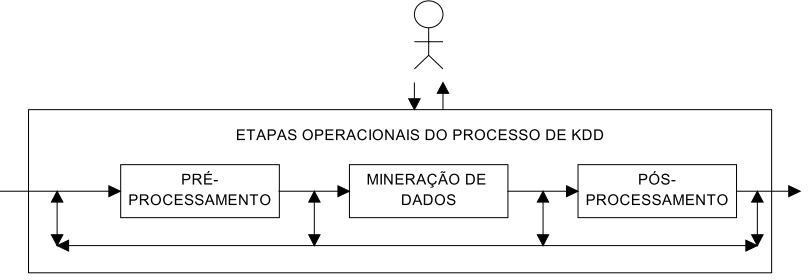
\includegraphics[scale=0.8]{images/KDD-macro.png}
	\caption{As macro etapas do processo de KDD. } 
	\small{Fonte: Boente, Goldschmidt e Estrela \citeyearpar{Boente-Goldschmidt}}
\end{figure}

Os autores Han e Kamber \citeyearpar{Han-kamber2nd} desenvolveram um processo de KDD baseando-se no proposto por Fayyad \textit{et al.} \citeyearpar{fayyad}. Nesse processo é possível visualizar o desmembramento das macro etapas citadas por Boente, Goldschmidt e Estrela \citeyearpar{Boente-Goldschmidt} em sete passos especializados, sendo: limpeza dos dados, integração dos dados, seleção dos dados, transformação dos dados, mineração de dados, avaliação de padrões e apresentação do conhecimento. A figura 2.2 traz a visão do processo de Han e Kamber \citeyearpar{Han-kamber2nd}.

\begin{figure}[!htb]
	\centering
	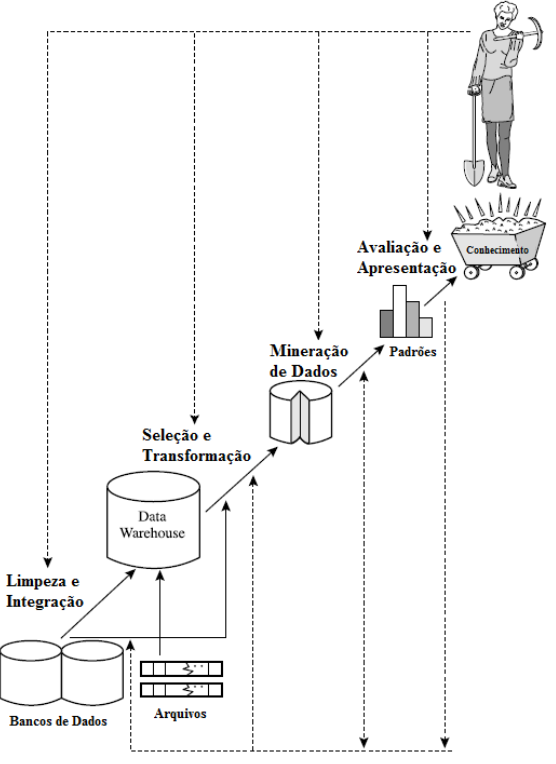
\includegraphics[scale=0.8]{images/HanKDD.png}
	\caption{O processo de KDD. } 
	\small{Fonte: Han e Kamber \citeyearpar{Han-kamber2nd}}
\end{figure}

\subsubsection{Pré-processamento dos dados}

O conhecimento obtido após o término oficial de um processo de KDD está intimamente ligado a qualidade dos dados de entrada. Todavia, se os dados presentes em grandes bases de dados e \textit{data warehouses} reais são inconsistentes, incompletos e com ruídos, conforme elenca Han e Kamber \citeyearpar{Han-kamber2nd}, então o conhecimento será de má qualidade. Fayyad \textit{et al.} \citeyear{fayyad} ainda salienta que a aplicação direta de mineração de dados, excluindo a etapa de pré-processamento, pode levar à descoberta de padrões sem sentido e inválidos. Larose \citeyearpar{larose2005} conclui dizendo que "para ser útil para fins da mineração de dados, os dados precisam passar por pré-processamento, na forma de limpeza e transformação de dados.".

A preparação dos dados para a mineração, denominado de pré-processamento por Han e Kamber \citeyearpar{Han-kamber2nd}, compreende os quatro primeiros passos, explicados, abaixo:

\textbf{Limpeza dos dados:} em Bancos de Dados, por exemplo, os dados tendem a ser incompletos e inconsistentes, assim, essa etapa visa a aplicação de métodos que eliminem essas incongruências de modo a não impactarem no resultado final. Essa etapa pode ser executada várias vezes sendo menos penosa quando se tem conhecimento acerca do domínio dos dados. Fayyad \textit{et al.} \citeyearpar{fayyad} elenca algumas operações básicas: remoção de ruídos, decisão de estratégias de gerenciamento de dados faltantes, entre outros. 

\textbf{Integração dos dados:} como o próprio nome sugere, integração compreende a etapa de integrar diferentes fontes de armazenamento de dados em um único repositório consistente. A partir disso, deve-se observar questões de redundância e dependência existentes entre atributos \cite{cassio-joao}.

\textbf{Seleção dos dados:} após a integração, se faz necessária a escolha dos atributos considerados importantes a partir da base de dados em estudo. Isso se faz importante, pois, embora a capacidade de processamento e memória tenha evoluído, o volume de dados é superior podendo inviabilizar a execução dos algoritmos para extração de padrões. \cite{rezende2003mineraccao}

\textbf{Transformação dos dados:} essa etapa merece atenção, pois alguns algoritmos trabalham apenas com valores numéricos e outros com valores categóricos \cite{cassio-joao}. Sendo assim, é necessária a transformação entre valores categóricos/numéricos de acordo com os objetivos pretendidos. Algumas etapas podem ser citadas para esse fim: suavização de dados discrepantes \textit{(outliers)}, agrupamento, generalização, normalização e a criação de novos atributos.


\subsubsection{Mineração de Dados}

A mineração de dados, em consonância com Hand, Mannila e Smith \citeyearpar{hand}, é "a análise de grandes conjuntos de dados a fim de encontrar relacionamentos inesperados e de resumir os dados de uma forma que eles sejam tanto úteis enquanto compreensíveis ao dono dos dados". Já na perspectiva de Cabena \textit{et al.} \citeyearpar{cabena}, a mineração de dados é "um campo multidisciplinar que reúne técnicas de aprendizagem de máquina, reconhecimento de padrões, estatísticas, banco de dados e visualização, para conseguir extrair informações de grandes bases de dados.". 

Neste trabalho entende-se mineração de dados como uma etapa do processo de KDD, pois existem etapas, anteriores e posteriores a mineração, muito importantes. Alguns defensores desse ponto de vista são Fayyad \textit{et al.} \citeyearpar{fayyad} que reafirmam "[...] KDD refere-se a todo o processo de descoberta de conhecimento e que mineração de dados compreende a aplicação de algoritmos específicos para a extração de padrões". 

Vale mencionar que mineração de dados não compreende uma simples consulta em um banco de dados ou, então, uma pesquisa na \textit{web}. Essas ações pertencem a área de recuperação de informação (\textit{information retrieval}) e não devem ser confundidas com mineração de dados \cite{pang-ning}. A etapa de mineração de dados será explorada com mais detalhes na seção 2.2.

\subsubsection{Pós-processamento dos dados}

Os passos seis e sete (avaliação de padrões e apresentação do conhecimento) do processo de KDD proposto por Han e Kamber \textit{et al.} \citeyearpar{Han-kamber2nd} agrupam-se na fase de pós-processamento de dados. Abaixo são detalhadas esses dois passos:

\textbf{Avaliação de padrões:} dependendo do resultado das etapas anteriores do processo de KDD, os algoritmos de mineração podem gerar um número elevado de padrões, dos quais muitos podem ser inúteis ao responsável pela execução do processo. Assim, Dantas \textit{et al.} \citeyearpar{dantas} diz que o passo de avaliação de padrões objetiva selecionar os padrões que fazem sentido com os objetivos pretendidos. 

\textbf{Apresentação de conhecimento:} a compreensão do conhecimento obtido é de suma importância, pois esse não é fornecido em uma saída perfeita e compreensível. Para tanto, são construídos relatórios, gráficos, interfaces \textit{web}, dentre outros que possibilitem o entendimento do conhecimento obtido \cite{brauner}. 

\section{Tarefas de Mineração de Dados}

As tarefas de mineração de dados são dividias em duas categorias: preditivas e descritivas. As preditivas preveem o valor de um atributo com base nos valores de outros atributos, as principais são: classificação e regressão. Já as tarefas descritivas visam a derivação de padrões (correlações, tendências, grupos) que sintetizem os relacionamentos subjacentes nos dados, sendo as principais: regras de associação e agrupamento \cite{pang-ning}. Assim, Larose \textit{et al.} \citeyearpar{larose2005} elenca as principais tarefas conforme explicado abaixo.

\textbf{Classificação:} "É o processo de encontrar um conjunto de modelos (funções) que descrevem e distinguem classes ou conceitos, com o propósito de utilizar um modelo para predizer a classe de objetos que ainda não foram classificados" \cite{amo2003}. A tarefa de classificação baseia-se na procura por um modelo capaz de determinar o valor do atributo classe em função dos valores dos demais atributos \cite{pang-ning}. Essa tarefa utiliza um conjunto de dados já classificados denominado conjunto de treinamento, através do qual são classificados novos objetos \cite{brauner}. Amo \citeyearpar{amo2003} dá como exemplo de aplicação de classificação descobrir se os clientes de um supermercado são bons ou maus compradores, por exemplo "clientes da faixa econômica B, com idade entre 50 e 60 anos são maus compradores". 

\textbf{Regressão:} é semelhante à classificação, no entanto é usada quando o atributo alvo é numérico ao invés de categórico. Fayyad \textit{et al.} \cite{fayyad} reforça o exposto salientando que a variável alvo assume um valor contínuo. Na regressão, novas observações são baseadas em um modelo de estimação que, por sua vez, advém dos valores de outras variáveis (demais atributos). Por exemplo, predizer a velocidade do vento (atributo alvo) em função da temperatura, umidade e pressão atmosférica \cite{pang-ning}.

\textbf{Regras de Associação:} visa descobrir as regras para quantificar a relação entre dois ou mais atributos. As regras de associação são da forma "SE atributo X ENTÃO atributo Y". Por exemplo, de 1000 clientes em um dia de semana a noite, de uma loja, 200 compraram fraldas e, desses 200, 50 compraram cervejas. Logo, a regra de associação poderia ser "Se comprou fraldas, então comprará cervejas" \cite{pang-ning}. As regras de associação serão melhor estudadas na seção 2.6

\textbf{Agrupamento:} objetiva colocar registros, observações ou classes de objetos similares dentro de grupos ou \textit{clusters} em inglês. Diferentemente das tarefas anteriores, o agrupamento não focaliza o valor de uma variável alvo. Em vez disso, segundo Larose \citeyearpar{larose2005}, "os algoritmos de agrupamento procuram segmentos definidos em subgrupos ou grupos relativamente homogêneos, onde a similaridade dos registros dentro do \textit{cluster} é maximizada e a similaridade fora é minimizada". Faceli \textit{et al.} \citeyearpar{faceli} aponta que existem vários algoritmos de agrupamento e que cada um emprega um critério impondo uma estrutura aos dados. Alguns exemplos de utilização de agrupamento, nas mais variadas áreas, são: processamento de imagens, pesquisa da mercado, reconhecimento de padrões. s

\section{Conselhos Municipais de Educação}

Os conselhos de educação não são recentes. Bordignon \citeyearpar{bordignon2009} diz que as tentativas de criação de conselhos de educação no Brasil remontam ao império, por volta de 1842 O Brasil conta com um conselho de educação de âmbito nacional funcionando efetivamente desde 1911, o qual veio evoluindo desde o ano citado. Entretanto, os Conselhos de âmbito municipal (CME) só tiveram um estímulo para sua criação após a criação dos sistemas municipais de ensino (SME) pela constituição Federal de \citeyearpar{const1988}, na qual, no Art. 211, explicita que a "União, os Estados, o Distrito Federal e os municípios organizarão, em regime de colaboração, seus sistemas de ensino."

O sistema de ensino remete a ideia de um todo, ou seja, "todas as atividades educacionais sob responsabilidade de um ente federado (União, Estado, Distrito Federal e Municípios) obedecem a um ordenamento legal e a uma estrutura administrativa oficial - o sistema de ensino" \cite{caderno-perfil}. Os conselhos de educação, hoje, fazem parte da estrutura de gestão dos sistemas de ensino e, se inexistente, priva o sistema ou a secretaria de educação de questões educacionais e de gestão participativa, democrática. Da mesma forma, existindo um conselho e inexistindo um sistema, esse último, por sua vez, limitará as atribuições do conselho. Isso acontece, pois a atual LDB (Lei de Diretrizes e Bases) nº 9.394 \citeyearpar{ldb}, em relação a Estados e Municípios, estabelece diretrizes somente para os sistemas de ensino, não fazendo referência aos conselhos de educação \cite{caderno-perfil}.

Bordignon \citeyearpar{bordignon2009} separa os conselhos em relação a natureza: consultivo, deliberativo ou outro. Tradicionalmente os conselhos exercem poderes de caráter consultivo e deliberativo. O primeiro assessora o governo nas ações referentes a área da educação. O segundo possui autonomia para estabelecer decisões sem a intervenção do poder executivo. Dada a natureza de um conselho, esse poderá exercer funções que seguem:

\begin{itemize}
	\item \textbf{Normativa:} tem caráter deliberativo e objetiva a normatização e regulação do sistema de ensino. É considerada uma das mais importantes atividades.
	\item \textbf{Interpretativa:} compreende a interpretação das normas de modo a ser capaz de sanar dúvidas (dos componentes do sistema) a respeito da correta aplicação de leis.
	\item \textbf{Credencialista:} também de caráter deliberativo, visa aprovar o credenciamento de novas instituições de ensino e cursos ofertados por essas. Em alguns casos, essa atividade abrange a aprovação de projetos político pedagógicos, regimentos e matrizes curriculares dos cursos.
	\item \textbf{Recursal:} propõe soluções de conflitos entre pais e instituições de ensino e dessas com o estado. 
	\item \textbf{Ouvidora:} defesa dos direitos educacionais dos cidadãos ouvindo-os e as instituições.
\end{itemize}

Os CME podem ser compostos por representantes de pais, professores, especialistas, entidades e órgãos ligados à educação municipal. O importante é que os membros sejam indicados de forma democrática. A democratização é muito importante, porém, a realidade é que muitos dos integrantes dos conselhos não possuem conhecimento suficiente para exercer as funções citadas anteriormente. Então, para isso, foram criados programas de formação no intuito de suprir essa deficiência e fortalecer os CME do Brasil.  \cite{cartilhaCruz}

\section{Ambiente de Mineração de Dados WEKA}

O \textit{Waikato Environment for Knowledge Analysis} (WEKA) é \textit{software} gratuito e \textit{open-source} que possui uma coletânea de algoritmos de aprendizado de máquina para tarefas de mineração de dados. O WEKA oferece um rol de funcionalidades que incluem pré-processamento de dados, classificação, regressão, \textit{clustering}, regras de associação e visualização. Foi desenvolvido na Nova Zelândia, em Java, na Universidade de Waikato e é distribuído sob a licença \textit{General Public License} - GNU. Ainda, é compatível com plataformas Windows, Linux e Mac OS \cite{weka}.

O WEKA permite aplicar algoritmos diretamente a conjuntos de dados através das seguintes interfaces: gráfica (comumente utilizada) ou código Java (Interface de Programação de Aplicativos, em inglês \textit{Application Programming Interface} - API). Dados podem ser importados diretamente de bases de dados via \textit{Java Database Connectivity driver} - JDBC. Vale lembrar que são aceitos arquivos de entrada no formato CSV e ARFF. Esse último é o formato padrão aceito pelo WEKA e será discutido na seção 2.5, além das vantagens e desvantagens no uso de um ou de outro. \cite{fischer} \cite{alcantara}.

Adotou-se o \textit{software} WEKA em razão dos conhecimentos prévios no uso da ferramenta, ser livre e por ser muito utilizada em estudos correlatos a proposta do presente trabalho. 

\section{O Formato ARFF}

O WEKA tem como entrada nativa arquivos do tipo ARFF, entretanto são aceitos arquivos do tipo CSV \cite{alcantara}. Esse último, em comparação com o formato ARFF possui desvantagens, pois o WEKA não consegue definir o tipo de dado em cada coluna e o usuário precisa informar ao programa essas informações no ato do carregamento do arquivo \cite{arff}. Vale salientar que arquivos CSV levam muito mais tempo para serem carregados comparados ao formato ARFF.

Um arquivo ARFF (\textit{Attribute-Relation File Format}) descreve uma lista de objetos que fazem uso de um conjunto de atributos. Um arquivo desse tipo possui duas seções em sua declaração, são elas: cabeçalho (\textit{header}) e dados (\textit{data}) \cite{arff}. O cabeçalho, por sua vez, ainda dividi-se em mais duas seções: \textit{Relation} e \textit{Attribute}. Em \textit{Relation} é definido o nome da relação cujo tipo é \textit{string}. 

Já na seção \textit{Attribute} são declarados todos os atributos (colunas de uma tabela relacional, por exemplo) com o seus respectivos tipos de dados. A ordem em que os atributos são declarados implica na ordem como os registros terão seus valores em cada coluna na seção \textit{data}. Um atributo, ao ser declarado, deve começar com uma letra e os tipos de dados suportados pelo WEKA são: númerico, nominal, \textit{string} e data \cite{libraga}.

Após o cabeçalho, segue-se com a seção de dados, onde são declarados. Para tanto, cada registro ocupa uma única linha sendo que os valores de cada coluna devem corresponder com a ordem e tipo de dado declarado na seção de atributos. Os valores faltantes são representados por um único ponto de interrogação \cite{arff}. A figura 2.3 apresenta a estrutura de um arquivo ARFF.

\begin{figure}[!htb]
	\centering
	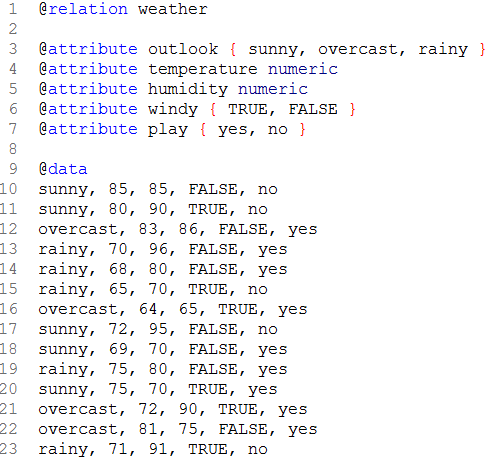
\includegraphics[scale=1]{images/arff.png}
	\caption{Estrutura do arquivo ARFF.} 
	\small{Fonte: Witten, Frank e Hall \citeyearpar{witten-hall}}
\end{figure}

A figura 2.3 exemplifica o que foi explicado, com um exemplo simples de dados meteorológicos. Na primeira linha é feita a declaração da relação \textit{weather} (tempo). Das linhas três a sete são declarados os atributos \textit{outlook, temperature, humidity, windy, play} (previsão, temperatura, umidade, ventoso e jogar respectivamente), cada um com seu tipo de dado. Os valores entre chaves apontam as únicas opções possíveis para um atributo. A partir da linha nove acontecem as definições de registros (dados) compostas por cinco colunas (já que cinco atributos foram declarados no cabeçalho).

\section{Regras de Associação}

A tarefa de associação prima encontrar elementos que implicam na presença de outros em uma mesma transação, em outras palavras, encontrar relacionamentos ou padrões frequentes entre conjuntos de dados \textit{itemsets}. Uma transação nada mais é que uma operação, por exemplo, uma compra que envolve a aquisição de produtos (itens) \cite{vasconcelos}.

Formula-se I = \{$i_1, ... ,i_m$\} como um conjunto de itens (produtos de um supermercado). Considera-se T = \{$t_1, ... ,t_n$\} um banco de dados de n transações (compras) sob I. Um subconjunto não vazio de I é considerado um \textit{itemset} e T suporta um \textit{itemset} I se I $\subseteq$ T. Desse modo, uma regra de associação é uma expressão da forma $A \rightarrow B$, onde A e B são \textit{itemsets}, por exemplo, $\{p\tilde{a}o, leite\} \rightarrow \{caf\acute{e}\}$. A ideia dessa regra é que pessoas que compram pão e leite tendem a comprar café, mas o contrário não é verdadeiro.\cite{amo2003}. Utilizando o exemplo de compras, um \textit{itemset} é um conjunto de produtos adquiridos por um cliente em uma compra (transação).

Cada regra na forma $A \rightarrow B$ possui dois parâmetros importantes que determinam sua validade para o conjunto de dados e auxiliam na delimitação da quantidade de regras extraídas: suporte e confiança \cite{gon}. O suporte de um \textit{itemset} A é a porcentagem de transações que contém A. O suporte de um \textit{itemset} é definido como:
\begin{gather*} 
suporte\ (A) = \frac{n\acute{u}mero\ de\ registros\ com\ (A)}{n\acute{u}mero\ total\ de\ registros}
\end{gather*}

O suporte de uma regra no formato $A \rightarrow B$ mostra-se, também, como uma porcentagem de transações que possuem A e B definido como:
\begin{gather*} 
suporte\ (A \cup B) = \frac{n\acute{u}mero\ de\ registros\ com\ (A \cup B)}{n\acute{u}mero\ total\ de\ registros}
\end{gather*}

Faceli \textit{et al.} \citeyearpar{faceli} define confiança como sendo o grau de interesse nas combinações de itens em que $A \cup B$ é um \textit{itemset} frequente. Esse grau de interesse consiste na probabilidade de ocorrer um conjunto de termos dado que ocorreu um outro conjunto, conforme a fórmula abaixo.
\begin{gather*} 
conf\ (A \rightarrow B) = \frac{suporte (A \cup B)}{suporte\ (A)}
\end{gather*} 

Dizer que uma regra de associação tenha um alto valor para o grau de confiança não garante que a mesma traga bons resultados. Isso acontece, pois a confiança pode referir-se às poucas transações que suportam a regra. Então, para garantir que uma dada regra $A \rightarrow B$ seja interessante é necessário exigir que seu valor de suporte também seja alto \cite{amo2003}

\section{Algoritmo Apriori}

O algoritmo \textit{Apriori} foi introduzido por Agrawal \textit{et al.} \citeyearpar{AgrawalIS93}; Agrawal e Srikant  \citeyearpar{AgrawalS94}, sendo o primeiro algoritmo para mineração de \textit{itemsets} e regras de associação. Segundo Faceli \textit{et al.} \citeyearpar{faceli} o algoritmo "utiliza uma estratégia de busca em largura, com um algoritmo de geração e teste. Em cada nível são gerados os \textit{itemsets} possíveis, tendo em conta os \textit{itemsets} frequentes gerados no nível anterior. Após serem gerados, a frequência desses \textit{itemsets} é testada, percorrendo novamente a base de dados de transações."

Com isso em vista, o algoritmo possui duas fases. A primeira é responsável por encontrar \textit{itemsets} frequentes e a segunda minerar regras de associação. A primeira etapa, sequenciada no algoritmo 1, resume-se em encontrar todos os \textit{itemsets} que possuem suporte acima do suporte mínimo $\sigma$, ou seja, os itens frequentes. 

A segunda fase, codificada no algoritmo 2, utiliza os itens frequentes para gerar as regras de associação. Por exemplo, considerando um conjunto de 5 itens frequentes \{café, pão, manteiga, leite, açúcar\} e um subconjunto de 2 itens frequentes \{café,  pão\}, pode-se obter uma regra do tipo (\{café, pão\} $\Longrightarrow$ \{leite, açúcar\}) respeitando a confiança (\{café, pão\} $\Longrightarrow$ \{leite, açúcar\}) $\ge$ confiança mínima definida pelo usuário.

A saída final do algoritmo, incluindo as duas fases, são regras de associação. Para facilitar o entendimento, a regra abaixo diz que se o café está barato então mais pães são comprados. Os valores 20 e 9 respectivamente indicam o número de registros onde café é barato e compra de pães é igual a "sim".

\begin{gather*} 
cafe = barato\ 20 \rightarrow p\tilde{a}es = sim\ 9\ conf(0.9)
\end{gather*} 

\begin{algorithm}[H]
	\Entrada{Um banco de dados de transações DB; Um limiar do suporte mínimo $\sigma$}
	\Saida{Todos os \textit{itemsets} com suporte maior que $\sigma$}
	\Inicio{
		Varrer o banco de dados uma vez\;
		Coletar $C_1$, o conjunto de itens frequentes e o suporte de cada item\;
		k $\leftarrow$ 1\;
		\Enqto{$C_k \neq$ vazio}{
			\ParaCada{transa\c{c}\~ao T $\in$ DB}{
				\ParaCada{\textit{itemset} candidato X $\in C_k$}{
					\Se{X $\in$ T}{
						Incrementa o suporte de X\;
					}
				}
			}
		}
		\tcc{Extrai todos os itemsets frequentes}
		$C_k \leftarrow \{X|X : Suporte \ge \sigma\}$\;
		\ParaCada{$X, Y \in C_k$}{
			\Se{X[i] = Y[i] para 1 $\ge i \ge$ k - 1eX[k] < Y[k]}{
				I = X $\cup$ \{Y[k]\}\;
				\Se{$\forall$ J $\in$ I, |J| = k : J $\in$ $C_k$}{
					$C_k+1 \rightarrow C_k+1 \cup I$
				}
			}
		}
		k $\leftarrow k + 1$\;
	}
	\caption{\textit{Apriori} para gerar \textit{itemsets} frequentes}
\end{algorithm} 


\begin{algorithm}[]
	\Entrada{\textit{Itemset} frequente I; Um limiar de confiança mínimo}
	\Saida{R: Todas as regras de associação em I com confiança maior que a confiança mínimo estabelecida}
	\Inicio{
	Gera todos os subconjuntos não vazios de I\;
	R = 0\;
	\ParaCada{subconjunto não vazio s de I}{
		Avalia a confiança da regra s $\rightarrow \{I/s\}$\;
		\Se{$\frac{suporte (I)}{suporte\ (s)} \ge confiança\ m\acute{i}n$  }{
			$R \rightarrow R \cup \{s \rightarrow \{I/s\}\}$
		}
	}
	}
	\caption{\textit{Apriori} para gerar regras de associação}
\end{algorithm} 

\chapter{Desenvolvimento}

Na intenção de atingir as expectativas deste estudo, serão consideradas três  tarefas globais: elaboração do dicionário de dados, construção do arquivo ARFF e aplicação do algoritmo de mineração de dados escolhido.  
O instrumento de coleta\footnote{Os dados foram coletadas através  de formulários do Google, onde cada linha da tabela representa uma resposta de um cursista com 43 atributos} da primeira edição do curso reuniu um total de 122 respostas, enquanto o da segunda 149 respostas totalizando um \textit{dataset} com 271 registros.

\section{Análise dos Dados}

Para melhor realizar a etapa de pré-processamento, é preciso entender o domínio dos dados. Para tal, foi construído um dicionário de dados (tabela 3.1) com quatro colunas. A primeira representa a pergunta do questionário (atributo); A segunda representa o tipo de variável, ou seja, se é categórica (qualitativa) ou numérica (quantitativa); A terceira representa o tipo de dado contido na variável (texto, data, inteiro ou opção); E a quarta representa a descrição do que o atributo armazena. 

O tipo de dado "opção" compreende uma faixa de valores possíveis. Por exemplo, o atributo "regional" pode ser populado com apenas um valor dentre 27 opções (siglas das regionais do RS). Outro exemplo denota-se pelo atributo "AtivCME", o qual pode assumir várias opções (um CME pode desenvolver mais de uma atividade). 

\begin{center}
	\begin{longtabu} to \textwidth {|c|c|c|X|} 
		\caption{Dicionário de dados}  \\
		\hline 
		atributo & tipo da variável & tipo de dado & descrição \\ \hline \hline
		nome & categórica & texto & nome do cursista \\ \hline
		papel & categórica & binário & função do cursista dentro do CME (conselheiro ou técnico) \\ \hline
		município & categórica & texto & cidade do RS \\ \hline
		regional & categórica & opção & regional da FAMURS (Composta por 27 Associações Regionais, a entidade representa todas as 497 cidades gaúchas). \\ \hline
		situacaoCME & categórica & opção & se o CME é ativo / inativo ou inexistente \\ \hline
		LeiMunicCriacCME & categórica & texto & descrição da lei de criação do CME \\ \hline
		dataCriacCME & categórica & data & data de criação do CME \\ \hline
		CMEfiliadoUNCME & categórica & binário & se o CME é ou não filiado a União Nacional dos Conselhos Municipais de Educação \\ \hline
		TemRegInterno & categórica & binário & se o CME possui ou não regimento interno \\ \hline
		QtdMembrosTit & numérica & inteiro & número de membros titulares que compõe o CME \\ \hline
		QtdMembrosSupl & numérica & inteiro & número de membros suplentes que compõe o CME \\ \hline
		EntdesOrgaRepCME & categórica & texto & entidades e órgãos com representação no CME atual \\ \hline
		SegRepPresViceCME & categórica & texto & segmento que representa o Presidente e o Vice do CME \\ \hline
		TemComIntern & categórica & binário & se o CME possui ou não comissões internas \\ \hline
		QtasComIntern & numérica & inteiro & quantidade de comissões internas  \\ \hline
		QtdreunioesMens & numérica & inteiro & quantidade de reuniões mensais \\ \hline
		QtdreunioesOrd & numérica & inteiro & quantidade de reuniões ordinárias \\ \hline
		QtdreunioesExtr & numérica & inteiro & quantidade de reuniões extraordinárias \\ \hline
		QtdOutrasReu & numérica & inteiro & quantidade de outros tipos de reuniões \\ \hline
		TemEspProprio & categórica & binário &  se possui ou não infra própria \\ \hline
		TipoEspaco & categorica & binário & se o espaço que possui é alugado ou conjugado com outro órgão \\ \hline
		QualOutroOrgao & categorica & texto & preencher o nome do outro órgão com o qual divide espaço \\ \hline 
		TemInternet & categórica & binário & se possui ou não acesso à internet \\ \hline  
		TemSiteBlogFace & categórica & binário & se possui mídia social \\ \hline  
		QualEndEle & categórica & texto & URL do site / blog / facebook  \\ \hline 
		PossuiGranaPropria & categórica & binário & se possui subsídios financeiros próprios \\ \hline
		DifRecursFinan & categórica & texto & descrição das dificuldades enfrentadas com os recursos financeiros \\ \hline 
		TemSME & categórica & binário & se possui ou não sistema municipal de ensino \\ \hline 
		DataCriacSME & categórica & data & data de criação do sistema municipal de ensino \\ \hline
		DocEmitCME & categórica & opção & documentos emitidos / deliberados pelo CME\\ \hline 
		PrincResoluc & categórica & texto & descrição de o que tratam as principais resoluções \\ \hline 
		PrincPareceres & categórica & texto & descrição de o que tratam os principais pareceres \\ \hline 
		MuncTemPNE & categórica & binário & se possui ou não plano municipal de educação \\ \hline    
		ComoPMECriado & categórica & texto & como o plano municipal de educação foi criado \\ \hline 
		QdoPMECriado & categórica & data & data de criação do plano de educação  \\ \hline 
		AtivCME & categórica & opção & principais atividades desenvolvidas pelo CME \\ \hline 
		ParticComConstMon & categórica & opção & Participa de Comissões de construção e/ou monitoramento e/ou assessoramento e/ou implementação de ... \\ \hline 
		DifculdEnfrentCME & categórica & opção & quais as principais dificuldades enfrentadas pelo CME no município \\ \hline 
		PossSolucDif & categórica & texto & quais as possíveis soluções para as dificuldades elencadas  \\ \hline 
		ProcUFSMAjudCME & categórica & texto & descrição se os estudos e discussões no curso Pró-Conselho estão ajudando no trabalho junto ao CME \\ \hline 
		ProcUsoAVEA & categórica & texto & descrição de quais são as percepções de quem está usando o AVEA - tecnologias educacionais para estudar \\ \hline 
		MelhorarProcUFSM & categórica & texto & sugestões de melhoria para o Pró-Conselho/UFSM \\ \hline 
	\end{longtabu}
\end{center}

 
\setlength{\baselineskip}{\baselineskip}

% Referências
\bibliography{referencias}
\bibliographystyle{abnt}


\end{document}
